% !TeX spellcheck = <none>
\documentclass[a4paper,12pt,onecolumn,oneside]{article}
\usepackage{cite}%bibTeX引用
\usepackage{ctex}
\usepackage{hyperref}%加入超链接
\usepackage{comment}
\usepackage{wrapfig}
\usepackage{graphicx}
\usepackage{float} 
\usepackage{amsmath}
\usepackage{amssymb}
\usepackage{geometry}
\geometry{a4paper,scale=0.8}
\usepackage{float}
\usepackage{subfigure} 
\usepackage{enumerate}%\item 需要
\usepackage{tabularx}% \table 
\usepackage{booktabs}% \toprule
\usepackage{tablefootnote}
\usepackage{longtable}
\usepackage{amsthm} %\qed
\usepackage{algorithm2e} %算法
\usepackage{booktabs}
\usepackage{longtable}
%%带颜色的表格%%
%\usepackage[table]{xcolor}
\usepackage{colortbl}
\definecolor{mygray}{gray}{.9}
\definecolor{mypink}{rgb}{.99,.91,.95}
\definecolor{mycyan}{cmyk}{.3,0,0,0}
%%带颜色的表格%%

\usepackage{titlesec}

% 在section标题前面加上一个§符号并居中
\titleformat{\section}
{\normalfont\Large\bfseries\centering}{\thesection}{1em}{}
%\titleformat{\subsection}
%{\normalfont\large\bfseries\centering}{\S\ \thesubsect\remove{text}ion}{1em}{}

%附录代码显示
\usepackage{listings,matlab-prettifier} % MATLAB 美化包
\lstset{
	style=Matlab-editor,
	numbers      = left,
	frame        = single,
}

\usepackage[T1]{fontenc}
\usepackage[utf8]{inputenc}
\usepackage{authblk}

\title{帆船价格数据集回归建模}
\author{第十组}
\date{}

\begin{document}
\section{绪论}
\subsection{数据及其背景}
帆船运动是一项广泛的兴趣爱好,但对于很多人来说,购买帆船是一笔不小的开支,所以相较于全新的帆船,二手帆船会受更多人的喜爱。然而,二手帆船的价格也会受出厂日期、长度、帆面积等影响。因此寻找帆船价格的影响因素至关重要。一方面这可以为二手帆船的售卖者提供合理定价的依据,从而增加出售量,另一方面这也可以为二手帆船的购买者提供购买思路,根据自己的习惯、喜好寻找价格合理的帆船。\par 
通过爬虫技术得到了帆船价格及其影响因素的1174条数据,数据说明如表\ref{tab:boat-variables}。\par 

\begin{table}[h]
	\centering
	\caption{帆船数据变量}
	\vspace{0.5\baselineskip}
	\label{tab:boat-variables}
	\begin{tabular}{|c|c|c|c|}
		\hline
		变量名 & 变量类型 & 取值范围 & 备注 \\ \hline
		ID & —— & Eg.Boat0001 & 帆船编号 \\ \hline
		Year & 连续型(自变量$x_1$) & [2005,2019] & 帆船出厂年份 \\ \hline
		Length & 连续型(自变量$x_2$) & [37.5,56] & 帆船长度 \\ \hline
		LWL & 连续型(自变量$x_3$) & [36.08,56.08] & 帆船设计水线长 \\ \hline
		Beam & 连续型(自变量$x_4$) & [19.67,24.21] & 帆船船宽 \\ \hline
		Draft & 连续型(自变量$x_5$) & [2.92,6.92] & 帆船吃水深度 \\ \hline
		Displacement & 连续型(自变量$x_6$) & [11000,77162] & 帆船排水量 \\ \hline
		SailArea & 连续型(自变量$x_7$) & [753,2626] & 帆船帆面积 \\ \hline
		GDP & 连续型(自变量$x_8$) & [0.6,3861] & 售卖地区的国内生产总值 \\ \hline
		GDP.Capita & 连续型(自变量$x_9$) & [2222,93667] & 售卖地区的人均国内生产总值 \\ \hline
		Price & 连续型(因变量$y$) & [95000,2890000] & 帆船的挂牌价格 \\ \hline
	\end{tabular}
\end{table}

\subsection{我们的任务}
建立因变量Price与Year、Length等9个自变量的模型,即定量分析9个自变量对因变量的影响。本文将建立线性回归模型、对数线性回归模型及广义线性模型,通过多重共线性、残差检验等对各个模型进行诊断并修正,最后通过预测准确率比较出最优模型。\par 

\subsection{主要选用方法——box-cox变换}
Box-Cox变换是Box和Cox在1964年提出的一种广义幂变换方法,是统计建模中常用的一种数据变换。回归模型建立有效的其中两个要求为残差,即因变量的真值与预测值的差,需满足正态分布,且有相同的方差,即方差齐性。若模型不满足,即可对因变量数据进行Box-Cox变换。Box-Cox变换公式为
$$
	y^{(\lambda)} =
	\begin{cases}
		\dfrac{(y_i^\lambda -1)}{\lambda} & \text{, 如果 } \lambda \neq 0 \\
		\ln(y_i) & \text{, 如果 } \lambda = 0
	\end{cases}
$$
其中$\lambda$的确定方法为,假设经过转换后的因变量就是服从正态分布的,然后画出关于$\lambda$的似然函数,似然函数值最大的时候$\lambda$的取值就是这里需要确定的值。
\subsection{主要函数说明及参数设置}
\begin{enumerate}
	\item 定义线性回归模型为
\begin{equation*}
	y=\beta_0+\beta_1 x_1+\beta_2 x_2+\beta_3 x_3+\beta_4 x_4+\beta_5 x_5+\beta_6 x_6+\beta_7 x_7+\beta_8 x_8+\beta_9 x_9
\end{equation*}
其中$\beta_0$为常数项,$\beta_i (i=1,2,...,9)$ 为第$i$个自变量的回归系数,应解释为当其他自变量不变时,$x_i$每变动一个单位因变量$y$的平均变动量。
\item 定义对数线性回归模型为
\begin{equation*}
	ln y=\beta_0+\beta_1 x_1+\beta_2 x_2+\beta_3 x_3+\beta_4 x_4+\beta_5 x_5+\beta_6 x_6+\beta_7 x_7+\beta_8 x_8+\beta_9 x_9
\end{equation*}
	其中$\beta_0$为常数项,$\beta_i (i=1,2,...,9)$为第$i$个自变量的回归系数。
	\item 定义广义线性回归模型为
	\begin{equation*}
		y = \beta_0 + \sum_{i=1}^{9}\sum_{j=1}^{k_i}\beta_{ij}x_i^j
	\end{equation*}
	其中$\beta_0$为常数项,$k$为第$i$个解释变量被拓展的最高次数,$\beta_{ij}$为第$i$个解释变量的$j$次方的回归系数。
	\end{enumerate}

	\section{线性回归模型}
	\subsection{异常值处理}
	利用R语言进行数据读入后可知此数据集由包含11个水平的1174条数据构成。剔除缺失值后对因变量绘制箱线图进行异常值检索,结果如图\ref{fig:tu21}所示。\par 
	\begin{figure}[h]
		\centering
		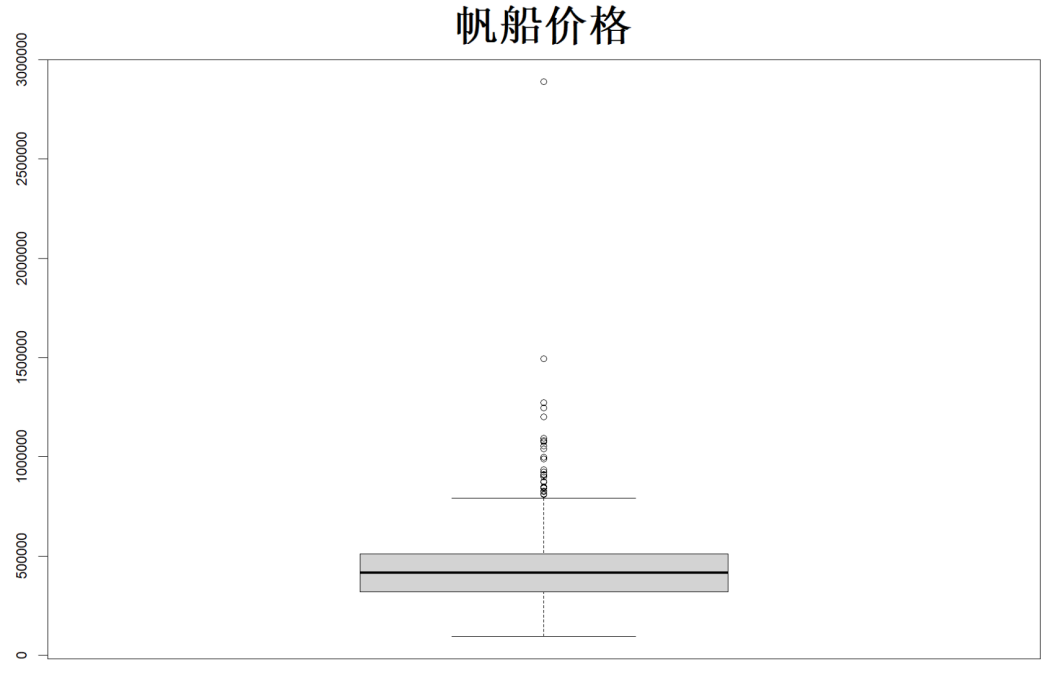
\includegraphics[width=0.8\textwidth]{res/tu21.png}
		\caption{帆船价格箱线图}
		\label{fig:tu21}
	\end{figure}
	如图所示,因变量存在较多离群点,考虑到数据量很大,因此删除离群点进行后续数据分析。另外,数据集中变量ID与后续数据分析无关,因此做删除处理。

	\subsection{模型建立与改进}
	\subsubsection{模型建立}
	以帆船价格为响应变量,其余所有变量为解释变量进行多元线性回归模型lm的建立,并对模型效果进行查看,结果如表\ref{tab:lm_analysis}所示。\par
\begin{table}[h]
	\centering
	\caption{lm相关参数分析}\vspace{0.3\baselineskip}
	\label{tab:lm_analysis}
	\begin{tabular}{@{}lccccc@{}}
		\toprule
		变量 & 估计系数 & 标准误 & t值 & p值 & 显著性 \\ \midrule
		常数 & $-3.950e+07$ & $1.208e+06$ & $-32.707$ & $< 2e-16$ & *** \\
		Length & $1.191e+04$ & $2.780e+03$ & $4.286$ & $2.01e-05$ & *** \\
		Year & $1.926e+04$ & $5.959e+02$ & $32.320$ & $< 2e-16$ & *** \\
		LWL & $8.397e+03$ & $2.615e+03$ & $3.211$ & $0.001369$ & ** \\
		Beam & $9.233e+03$ & $3.135e+03$ & $2.946$ & $0.003305$ & ** \\ 
		Draft & $-1.040e+04$ & $7.325e+03$ & $-1.419$ & $0.156201$ &  \\
		Displacement & $-8.517e-01$ & $4.848e-01$ & $-1.757$ & $0.079312$ & . \\
		SailArea & $9.039e+01$ & $2.621e+01$ & $3.449$ & $0.000589$ & *** \\
		GDP & $1.439e+01$ & $2.953e+00$ & $4.871$ & $1.31e-06$ & *** \\
		\bottomrule
	\end{tabular}
\end{table}
\pagebreak
\begin{table}[h]
	\centering
	\begin{tabular}{@{}lccccc@{}}
		\toprule
		变量 & 估计系数 & 标准误 & t值 & p值 & 显著性 \\ \midrule

		GDP.Capita & $2.695e-01$ & $1.923e-01$ & $1.401$ & $0.161431$ &  \\ \midrule
		R$^2=0.7292$ & \multicolumn{2}{c}{调整R$^2=0.7266$} & F(9,916)=274.1 & \multicolumn{2}{c}{p<2.2e-16} \\ \bottomrule
	\end{tabular}
\end{table}

分析上述表格,由$R^2$和调整$R^2$值接近于1,可知本模型拟合效果良好,且p值小于0.05,说明在检验水平为0.05条件下,因变量与其他变量之间的线性关系显著。观察各变量的拟合系数知,存在部分变量进行模型效果不显著的问题,因此考虑以逐步回归进行模型改进。
	\subsection{模型改进}
对上述模型lm进行逐步回归形成新模型lm.aic,经对比可知模型lm.aic在原模型基础上剔除变量Draft和GDP.Capita。为检验解释变量之间相关性对模型的影响,现运用方差膨胀因子法对本模型进行多重共线性诊断,当vif<10时,我们可认为自变量之间不存在多重共线性,当vif>10时,我们认为自变量之间存在严重的多重共线性,检验结果如下:\par 
\begin{table}[htbp]
	\centering
	\caption{方差膨胀因子法}\vspace{0.5\baselineskip}
	\label{tab:vif}
	\begin{tabular}{@{}lccccccc@{}}
		\toprule
		变量 & Length & Year & LWL & Beam & Displacement & GDP & SailArea \\
		vif值 & 18.19 & 1.24 & 10.66 & 4.70 & 5.94 & 1.01 & 7.67 
		\\\bottomrule
	\end{tabular}
\end{table}
由检验结果知,变量Length与LWL之间存在严重的多重共线性,且Length的vif值最大,因此考虑将其从模型中移除,进行重新建模lm1。下面将展示对模型lm1潜在问题的诊断及修正过程。
\subsection{模型诊断}
\subsubsection{整体诊断}
绘制线性模型的整体散点图进行模型整体分析。观察\ref{fig:tu231}中左下图可知散点分布不随机,具有近似二次曲线的趋势,因此可认为模型残差存在异方差。观察Q-Q图可知,随横坐标增大,散点分散近似成一条直线,因此可认为残差服从正态分布;观察右下图可知存在较多离群点。因此得出结论,本模型存在较大改进空间,下面将进行逐一诊断与改进。
	\begin{figure}[H]
	\centering
	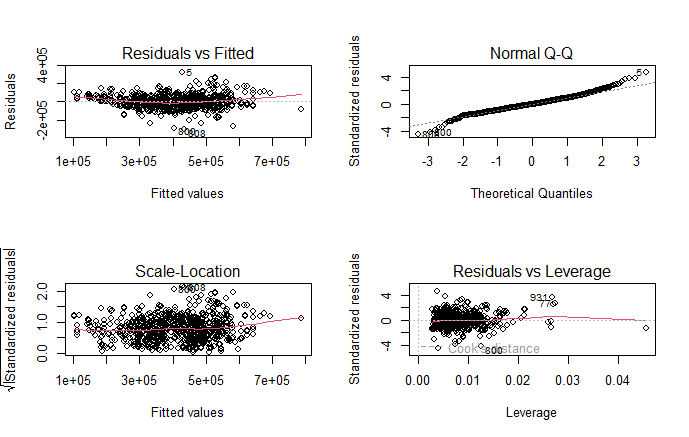
\includegraphics[width=\textwidth]{res/tu231.png}
	\caption{模型诊断图}
	\label{fig:tu231}
\end{figure}
\subsubsection{残差正态性检验}
由上面残差Q-Q图可直观判断,残差服从正态分布,下面针对模型lm1的标准化残差进行K-S检验,检验结果如下。\par 
\begin{table}[htbp]
	\centering
	\caption{K-S检验}\vspace{0.5\baselineskip}
	\label{tab:ks_test}
	\begin{tabular}{@{}ccc@{}}
		\toprule
		检验变量 & 统计量D值 & P值 \\
		\midrule
		lm1模型残差(标准化) & 0.036719 & 0.1646 \\
		\bottomrule
	\end{tabular}
\end{table}
由检验结果,检验p值并不显著,因此在检验水平为0.05条件下不能拒绝原假设,即模型lm1的标准化残差服从正态分布。
\subsubsection{方差齐性检验}
\begin{enumerate}
	\item 异方差检验\par 整体检验时已经分析残差图,散点随横坐标呈现一定趋势,随机性较差,因此直观认为残差之间存在异方差,下面对改进后的模型采用ncv计分检验,当检验显著时可认为存在异方差,检验结果如下表。
	\begin{table}[htbp]
		\centering
		\caption{ncv检验}\vspace{0.5\baselineskip}
		\label{tab:ncv_test}
		\begin{tabular}{@{}lccc@{}}
			\toprule
			检验变量 & Chisquare & df & p \\
			\midrule
			lm1 & 26.9441 & 1 & 2.0943e-07 \\
			\bottomrule
		\end{tabular}
	\end{table}
	由检验p值小于0.05可认为检验显著,则认为存在异方差,需进行模型修正。
	\item box-cox变换 \par 由上述检验结果知改进的模型存在异方差问题,基于此考虑将数据进行广义box-cox变换改进数据的形态,而此变换重点在于寻求合适的参数$\lambda$,使由模型得到的似然函数取到极大值,下图即为确定$\lambda$的过程。
	\begin{figure}[H]
	\centering
	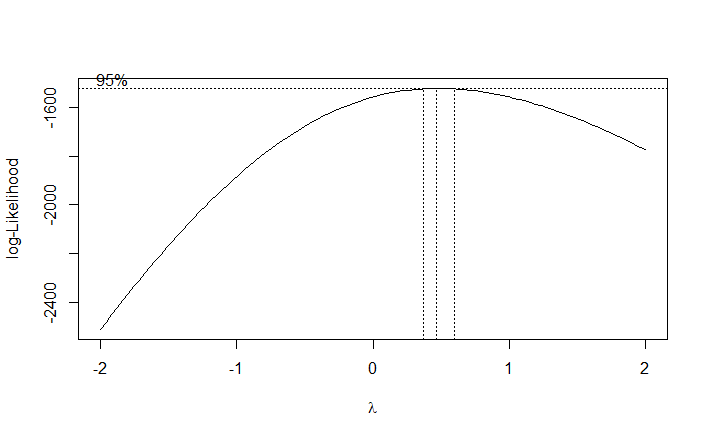
\includegraphics[width=\textwidth]{res/tu2.3.3.png}
	\caption{$\lambda$极大似然函数图}
	\label{fig:tu2.3.3}
\end{figure}
由图可看出,对数似然函数单调递增,只能在给定区间确定极大值。本次变换中即取$\lambda=0.4646465$代入公式
\begin{equation}\label{eq:1}
	y^{*} = \frac{(y^{\lambda}-1)}{\lambda}
\end{equation}
得到新的因变量$y^{*}$进行重新建模得新模型(lm2),再次对模型残差进行方差齐性检验,发现异方差问题已解决,同时对新模型再次进行残差正态性检验,发现正态性更加良好,说明本次变换取得一定效果。
\end{enumerate}
\subsubsection{多重共线性诊断}
运用方差膨胀因子法对模型lm2进行多重共线性诊断,结果如下:\par
\begin{table}[htbp]
	\centering
	\caption{方差膨胀因子法}\vspace{0.5\baselineskip}
	\label{tab:vif_test}
	\begin{tabular}{@{}lcccccc@{}}
		\toprule
		变量 & Year & LWL & Beam & Displacement & GDP & SailArea \\
		\midrule
		vif值 & 1.19 & 5.21 & 4.09 & 4.75 & 1.01 & 7.54 \\
		\bottomrule
	\end{tabular}
\end{table}
由检验结果知,各解释变量之间不存在严重的多重共线性,即多重共线性检验通过。
\subsection{模型应用}
经上述检验,可确定最终模型lm2,对其效果进行查看,结果如下。
\begin{table}[htbp]
	\centering
	\caption{lm2相关参数分析}\vspace{0.5\baselineskip}
	\begin{tabular}{llllll}
		\toprule
		变量 & 估计系数 & 标准误 & t值 & p值 & 显著性 \\
		\midrule
		常数 & -3.748e+04 & 1.168e+03 & -32.076 & $< 2e-16$ & *** \\
		Year & 1.848e+01 & 5.764e-01 & 32.014 & $< 2e-16$ & *** \\
		LWL & 1.345e+01 & 1.791e+00 & 7.510 & 1.40e-13 & *** \\
		Beam & 2.073e+01 & 2.881e+00 & 7.195 & 1.30e-12 & *** \\
		Displacement & 1.578e-04 & 4.253e-04 & 0.371 & 0.710622 & \\
		SailArea & 9.003e-02 & 2.453e-02 & 3.670 & 0.000257 & *** \\
		GDP & 1.807e-02 & 2.507e-03 & 7.207 & 1.19e-12 & *** \\
		\midrule
		$R^2=0.738$ & \multicolumn{5}{l}{调整$R^2=0.7363$ $F(6,916)=431.5$ $p<2.2e-16$} \\
		\bottomrule
	\end{tabular}%
	\label{tab:lm2}%
\end{table}
由上述数据展示,$R^2$与调整$R^2$有较大提升,p值仍旧显著,证明模型的修正取得良好成效,模型可靠度很高。建模最终得到回归方程
\begin{align}\label{eq:2}
	y^{*} &= (-3.748e+04) + (1.848e+01) x_1 + (1.345e+01) x_3 + (2.073e+01) x_4 \nonumber \\
	&\quad + (1.578e-04) x_6 + (9.003e-02) x_7 + (1.807e-02) x_8
\end{align}
基于上述模型,当给定解释变量值,即可代入公式(\ref{eq:2})较为可靠的计算出因变量值,但这里求得的是变换后的值,并非实际因变量值,再由公式(\ref{eq:1})可反解得
\begin{equation}
	y = (\lambda y^{*}+1)^{\frac{1}{\lambda}}
\end{equation}
代入此公式即可求得真实因变量的值。\par 
定义预测错误率为
\begin{equation}\label{eq:4}
	r = \frac{\sum_{i=1}^{n}|\frac{y_i-\hat{y_i}}{y_i}|}{n}
\end{equation}
其中$r$为预测错误率,$y_i$为因变量的真实值,$\hat{y_i}$为因变量的预测值,$n$为数据量。其本质为每条数据预测错误率的均值。\par 
将自变量的数据代入(\ref{eq:2})中,并进行Box-Cox逆变换,得到因变量的预测值,并将所需数据代入(\ref{eq:4})中,得到线性回归模型的预测错误率r=12.22\%,可见此线性回归模型对数据有一定的预测准确性,但仍需改进。

\section{对数线性回归模型}
\subsection{异常值处理}
将961条数据读入后将price值取对数得到因变量,剔除缺失值后,对因变量绘制箱线图进行异常值检索,结果如下。\par 
	\begin{figure}[H]
	\centering
	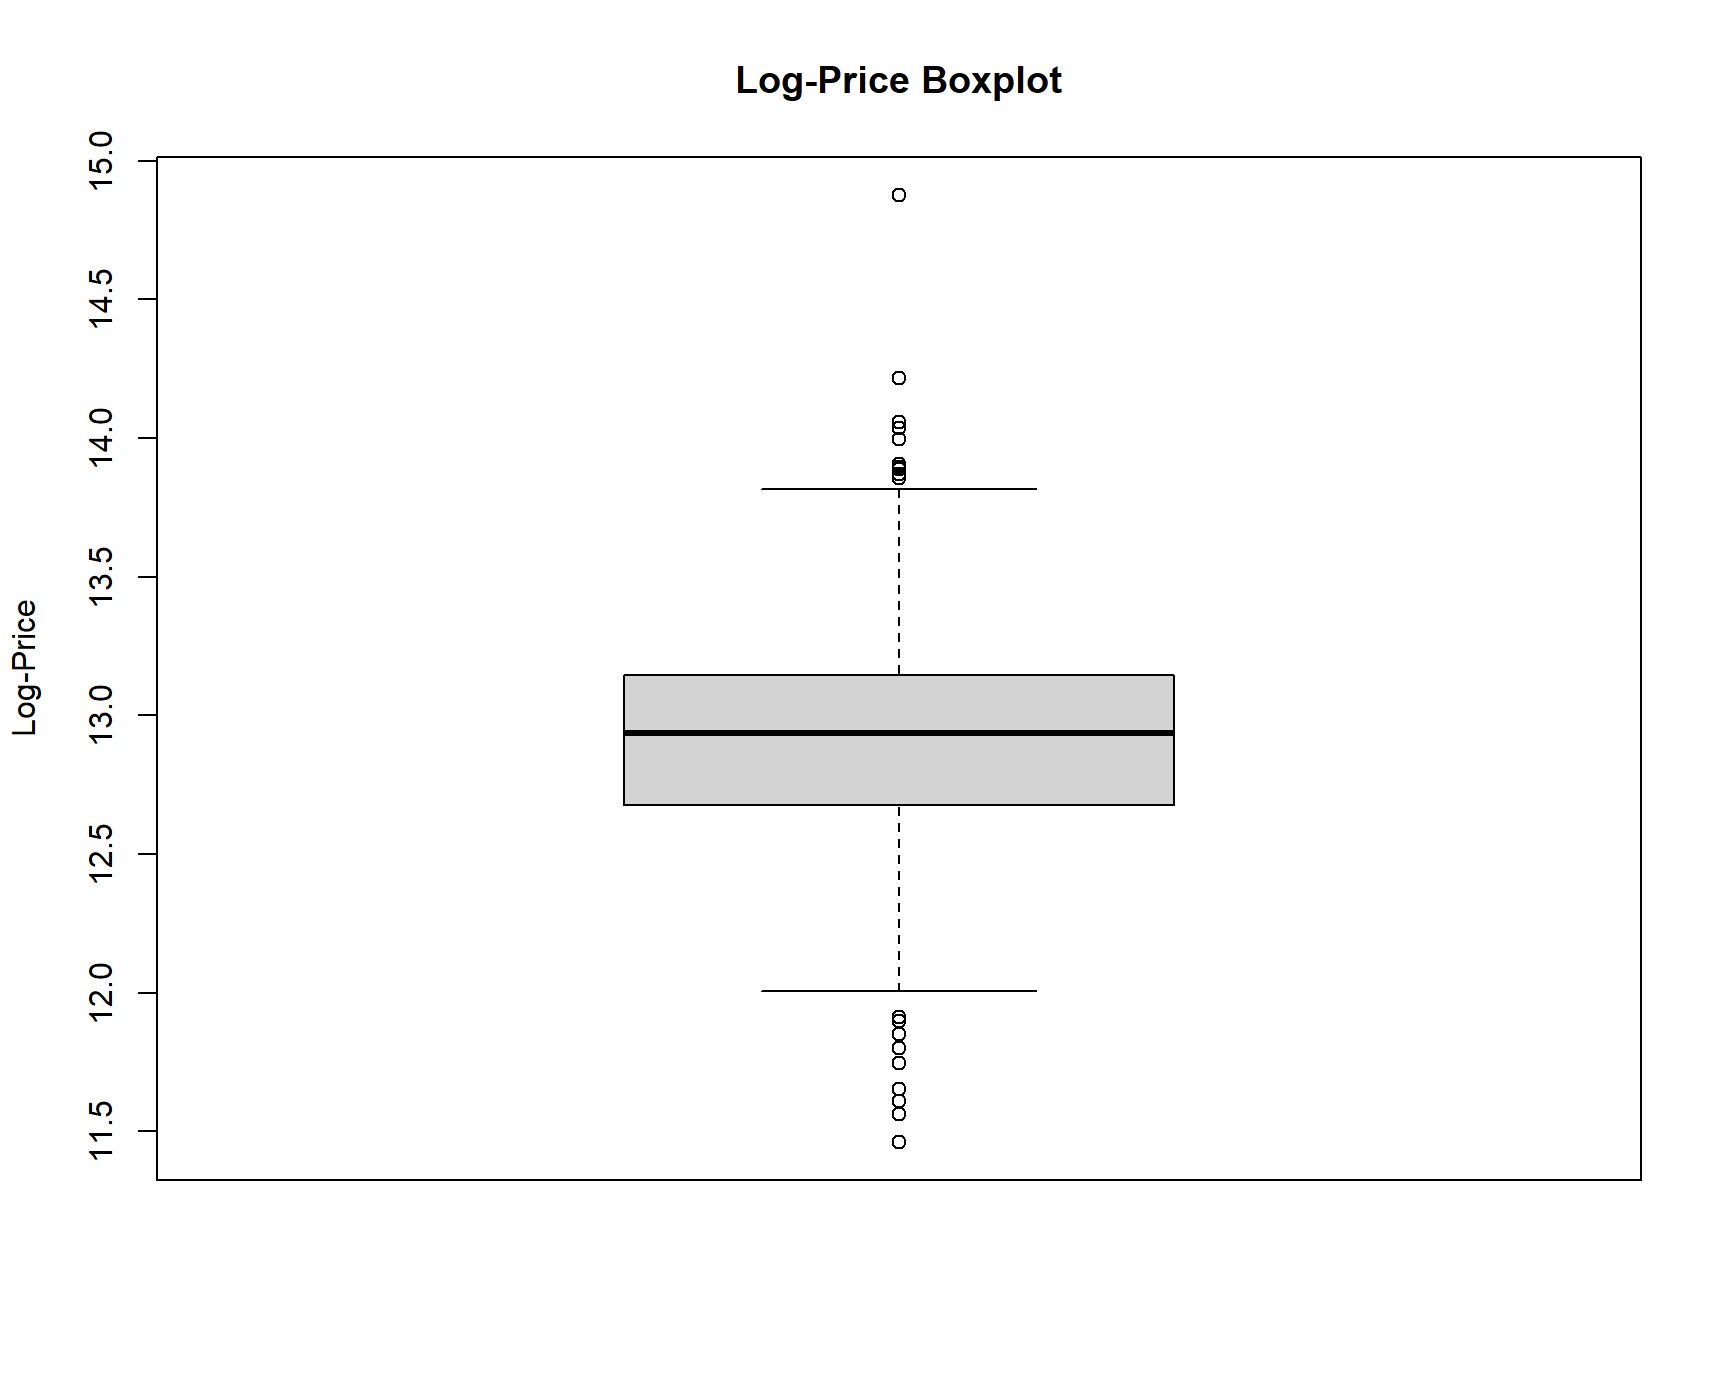
\includegraphics[width=0.73\textwidth]{res/box.png}
	\caption{帆船对数价格箱线图}
	\label{fig:box}
\end{figure}
删除离群点后共941条数据。同样地,数据集中变量ID与后续数据分析无关,因此做删除处理。
\subsection{模型建立}
以帆船价格的对数为响应变量,其余所有变量为解释变量进行对数线性回归模型model的建立,并对模型效果进行查看,结果如下。
\begin{table}[htbp]
	\centering
	\caption{model相关参数分析}\vspace{0.5\baselineskip}
	\begin{tabular}{llllll}
		\toprule
		变量 & 估计系数 & 标准误 & t值 & p值 & 显著性 \\
		\midrule
		常数 & -9.059e+01 & 2.685e+00 & -33.745 & $<$ 2e-16 & *** \\
		Length & 3.190e-02 & 5.593e-03 & 5.705 & 1.57e-08 & *** \\
		Year & 4.977e-02 & 1.327e-03 & 37.515 & $<$ 2e-16 & *** \\
		LWL & 1.748e-02 & 5.629e-03 & 3.105 & 0.00196 & ** \\
		Beam & 3.817e-02 & 7.128e-03 & 5.355 & 1.08e-07 & *** \\
		Draft & 2.631e-02 & 1.565e-02 & 1.681 & 0.09302 & . \\
		Displacement & -1.917e-06 & 1.025e-06 & -1.871 & 0.06172 & . \\
		SailArea & 1.301e-04 & 5.631e-05 & 2.310 & 0.02108 & * \\
		GDP & 3.811e-05 & 6.731e-06 & 5.662 & 1.99e-08 & *** \\
		GDP.Capita & 1.299e-06 & 4.434e-07 & 2.930 & 0.00347 & ** \\
		\midrule
		\multicolumn{6}{l}{R$^2$=0.7887 调整R$^2$=0.7866 F(9,931)=386.1 p$<$2.2e-16} \\
		\bottomrule
	\end{tabular}%
	\label{tab:addlabel}%
\end{table}
分析上述表格,由$R^2$和调整$R^2$值接近于1,可知本模型拟合效果良好,且p值小于0.05,说明在检验水平为0.05条件下,因变量与其他变量之间的线性关系显著。
\subsection{模型改进}
运用方差膨胀因子法对本模型进行多重共线性诊断,检验结果如表\ref{tab:vif2}所示。\par 
\begin{table}[htbp]
	\centering
	\caption{方差膨胀因子}\vspace{0.5\baselineskip}
	\begin{tabular}{c|ccccc}
		\toprule
		& \multicolumn{5}{c}{独立变量} \\
		\cmidrule{2-6}          & Length & Year  & LWL   & Beam  & Draft \\
		\hline
		vif值  & 15.04 & 1.17  & 10.40 & 4.51  & 1.49 \\\midrule
		& Displacement & SailArea & GDP   & GDP.Capita &  \\\hline 
		vif值  & 5.10  & 7.90  & 1.01  & 1.41  &  \\
		\bottomrule
	\end{tabular}%
	\label{tab:vif2}%
\end{table}%
由检验结果知,变量Length与LWL之间存在严重的多重共线性,且Length的vif值最大,因此考虑将其从模型中移除,进行重新建模得到model1。下面将展示对模型model1潜在问题的诊断及修正过程。
\subsection{模型诊断}
\subsubsection{整体诊断}
	\begin{figure}[H]
	\centering
	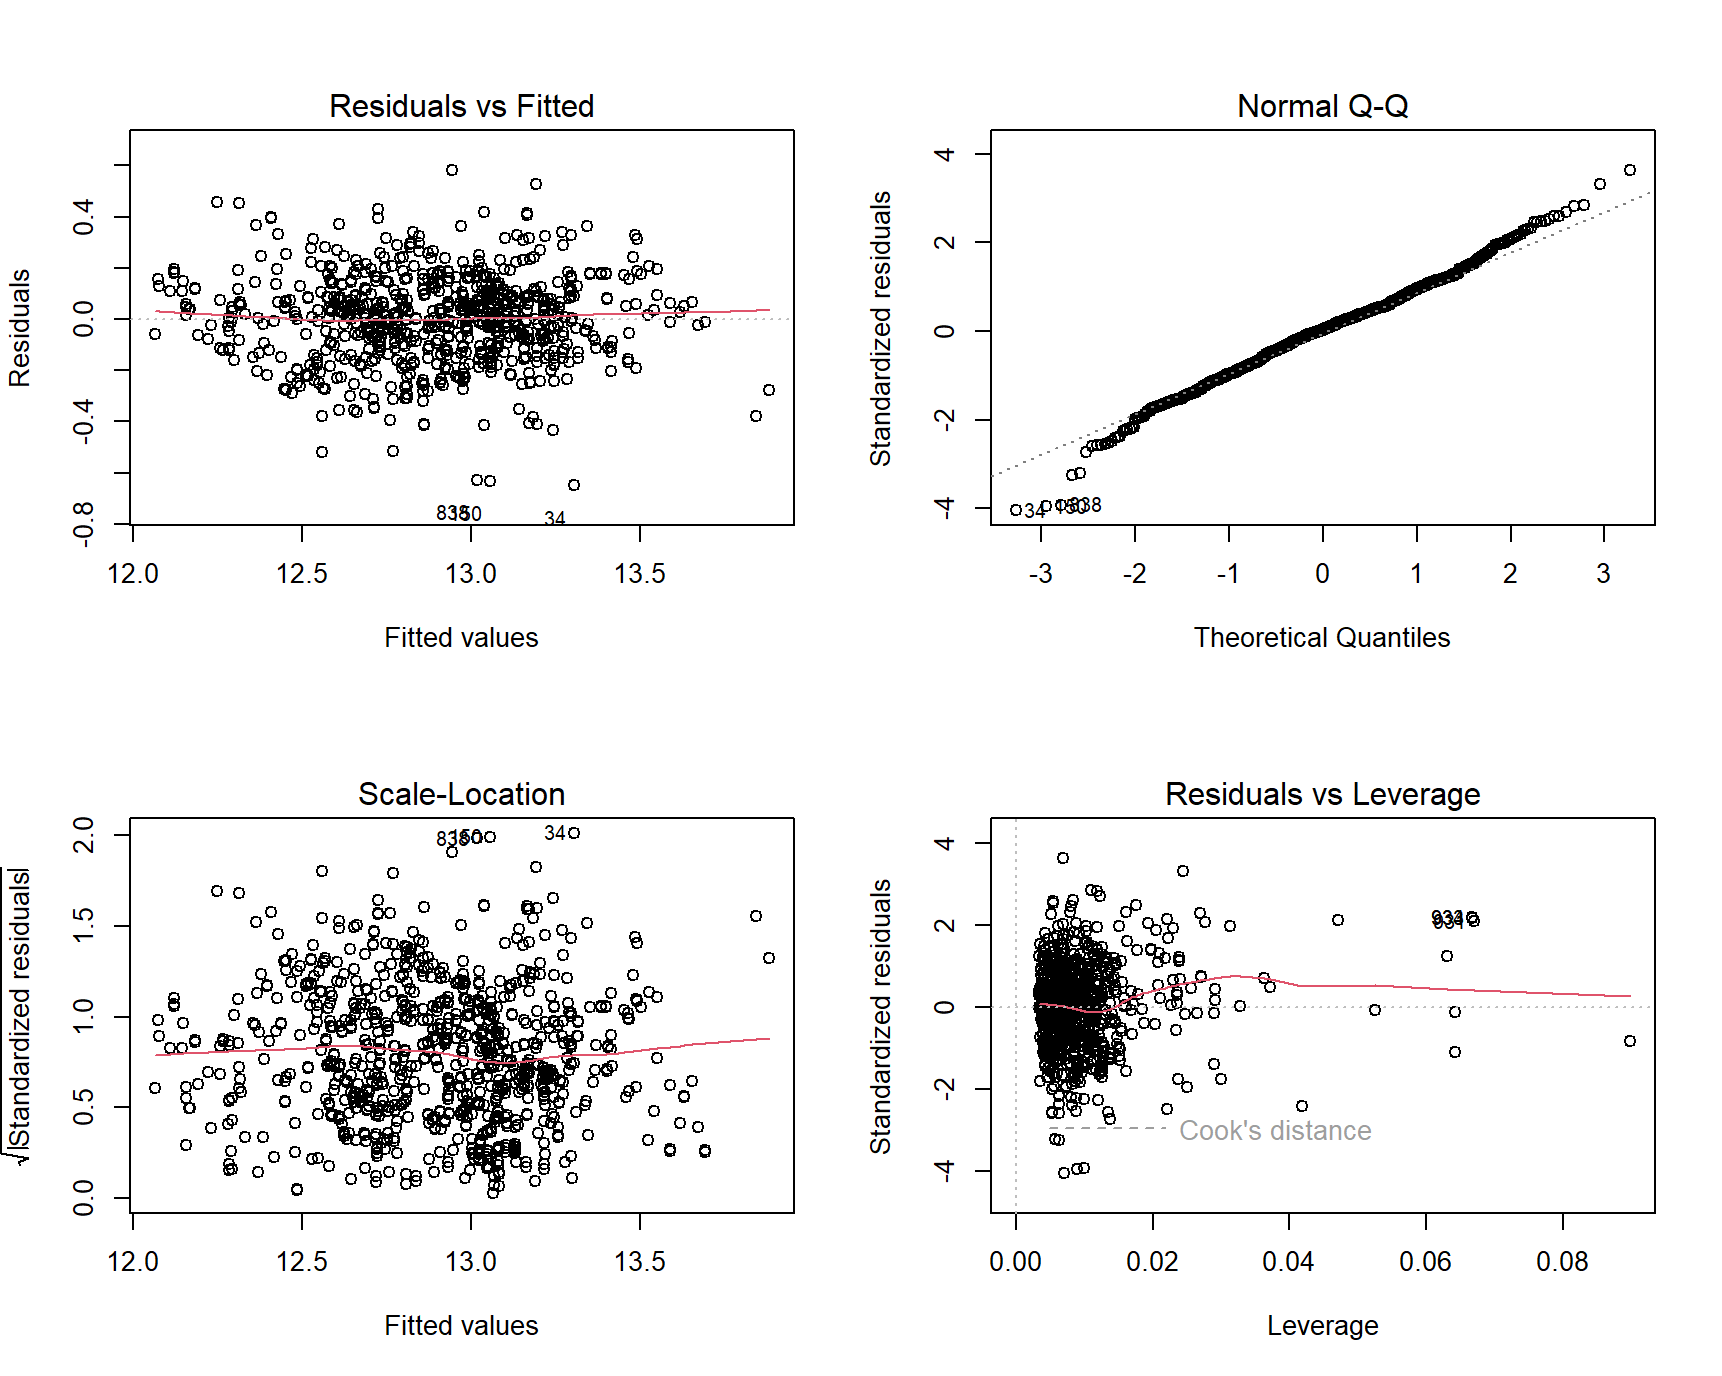
\includegraphics[width=0.8\textwidth]{res/zhenduan.png}
	\caption{模型诊断图}
	\label{fig:zhengti}
\end{figure}
绘制线性模型的整体散点图进行模型整体分析。观察左下图可知散点分布基本随机;观察Q-Q图可知,随横坐标增大,散点分散近似成一条直线,因此可认为残差服从正态分布;观察右下图可知存在较多离群点。下面将对模型进行检验。
\subsubsection{残差正态性检验}
由上面残差Q-Q图可直观判断,残差服从正态分布,下面针对模型model1的标准化残差进行K-S检验,检验结果如下。\par 
\begin{table}[h]
	\centering
	\caption{K-S检验}\vspace{0.25\baselineskip}
	\begin{tabular}{ccc}
		\toprule
		检验变量 & 统计量D值 & P值 \\
		\midrule
		lm1模型残差(标准化) & 0.035694 & 0.1817 \\
		\bottomrule
	\end{tabular}
\end{table}
由检验结果,检验p值并不显著,因此在检验水平为0.05条件下不能拒绝原假设,即模型model1的标准化残差服从正态分布。
\subsubsection{方差齐性检验}
由整体检验时已经分析残差图,散点随机性较良好,因此直观认为残差之间不存在异方差,对模型采用ncv计分检验,检验结果如下表。\par 
\begin{table}[h]
	\centering
	\caption{ncv检验}\vspace{0.25\baselineskip}
	\label{tab:ncv}
	\begin{tabular}{ccc c}
		\toprule
		检验变量 & Chisquare & df & p \\
		\midrule
		lm1 & 1.399706 & 1 & 0.23677 \\
		\bottomrule
	\end{tabular}
\end{table}
由检验p值大于0.05可认为检验不显著,则认为不存在异方差。
\subsubsection{多重共线性诊断}
运用方差膨因子法对模型model1进行多重共线性诊断,结果如下:\par 
\begin{table}[h]
	\centering
	\caption{方差膨胀因子法}\vspace{0.25\baselineskip}
	\begin{tabular}{ccccccccc}
		\toprule
		变量 & Year & LWL & Beam & Displacement & GDP & SailArea & Draft & GDP.Capita \\\hline
		vif值 & 1.14 & 5.53 & 4.07 & 4.36 & 1.39 & 7.77 & 1.49 & 1.41 \\
		\bottomrule
	\end{tabular}
\end{table}
由检验结果知,各解释变量之间不存在严重的多重共线性,即多重共线性检验通过。
\subsection{模型应用}
经上述检验,可确定最终模型model1,对其效果进行查看,结果如下。\par 
\begin{table}[h]
	\centering
	\caption{model1相关参数分析}\vspace{0.25\baselineskip}
	\label{tab:model1}
	\begin{tabular}{@{}llllll@{}}
		\toprule
		变量 & 估计系数 & 标准误 & t值 & p值 & 显著性 \\ \midrule
		常数 & -8.821e+01 & 2.696e+00 & -32.714 & $<$ 2e-16 & *** \\
		Year & 4.859e-02 & 1.332e-03 & 36.467 & $<$ 2e-16 & *** \\
		LWL & 3.947e-02 & 4.171e-03 & 9.463 & $<$ 2e-16 & *** \\
		Beam & 5.093e-02 & 6.882e-03 & 7.400 & 3.03e-13 & *** \\
		Draft & 3.092e-02 & 1.589e-02 & 1.946 & 0.05192 & . \\
		Displacement & 3.081e-07 & 9.639e-07 & 0.320 & 0.74927 & \\
		SailArea & 1.716e-04 & 5.678e-05 & 3.023 & 0.00257 & ** \\
		GDP & 3.952e-05 & 6.840e-06 & 5.778 & 1.03e-08 & *** \\
		GDP.Capita & 1.287e-06 & 4.509e-07 & 2.856 & 0.00439 & ** \\ \midrule
		R$^2$=0.7813 & 调整R$^2$=0.7794 & F(8,932)=416.2 & p$<$2.2e-16 & & \\
		\bottomrule
	\end{tabular}
\end{table}
由于$R^2$与调整$R^2$的值会随着变量个数的减少而减小,model1的$R^2$和调整$R^2$略低于改进前模型model,而model1的$R^2$和调整$R^2$均大于线性回归模型lm2,且p值仍旧显著,证明模型基本可靠。建模最终得到回归方程
\begin{align}
	ln y^{*} &=(-8.821e+01)+(4.859e-02) x_1+(3.947e-02) x_3+(5.093e-02) x_4 \nonumber \\
	&\quad +(3.092e-02) x_5+(3.081e-07) x_6+(1.716e-04) x_7+(3.952e-05) x_8 \nonumber \\
	&\quad+( 1.288e-06) x_9
\end{align}
该模型输出的因变量为价格的对数,在进行预测错误率计算之前,需要将其通过指数函数转化为价格数据,以此代入(\ref{eq:4})进行计算。计算出该对数线性回归模型的预测错误率为r=12.50\%,相较于线性回归模型没有改善。
\section{广义线性回归模型}
\subsection{异常值处理}
将 961 条数据读入后将 Price 值取对数得到新相应变量 Log\_Price,剔除缺失值后,对 Log\_Price 绘制箱线图进行异常值检索,结果如下。
	\begin{figure}[H]
	\centering
	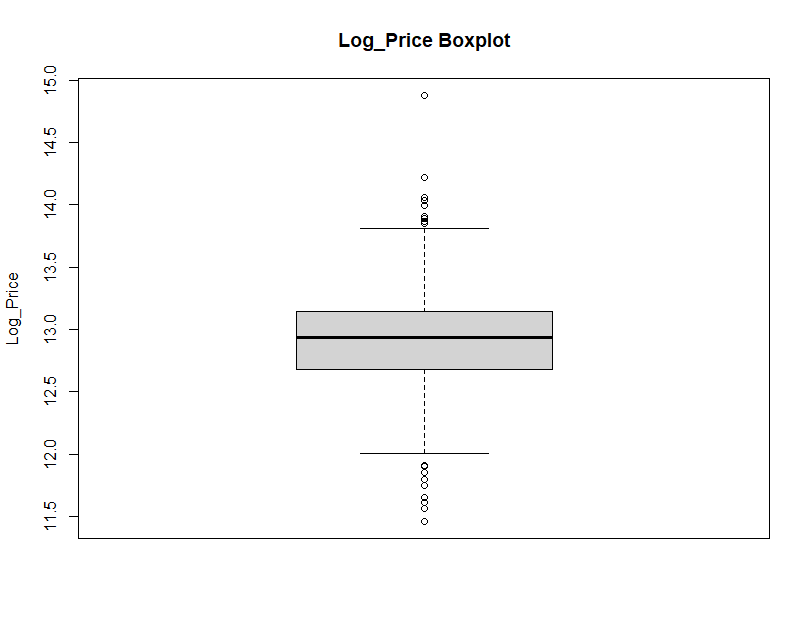
\includegraphics[width=0.6\textwidth]{res/yichang.png}
	\caption{帆船对数价格箱线图}
	\label{fig:box2}
\end{figure}
删除离群点后共 941 条数据。同样地,数据集中变量 ID 与后续数据分析无关,因此做删除处理。
\subsection{模型建立}
以 Log\_Price 为响应变量,分别以每一个变量为解释变量先进行简单的线性回归,并观察数据的分布,图像如下:
	\begin{figure}[H]
	\centering
	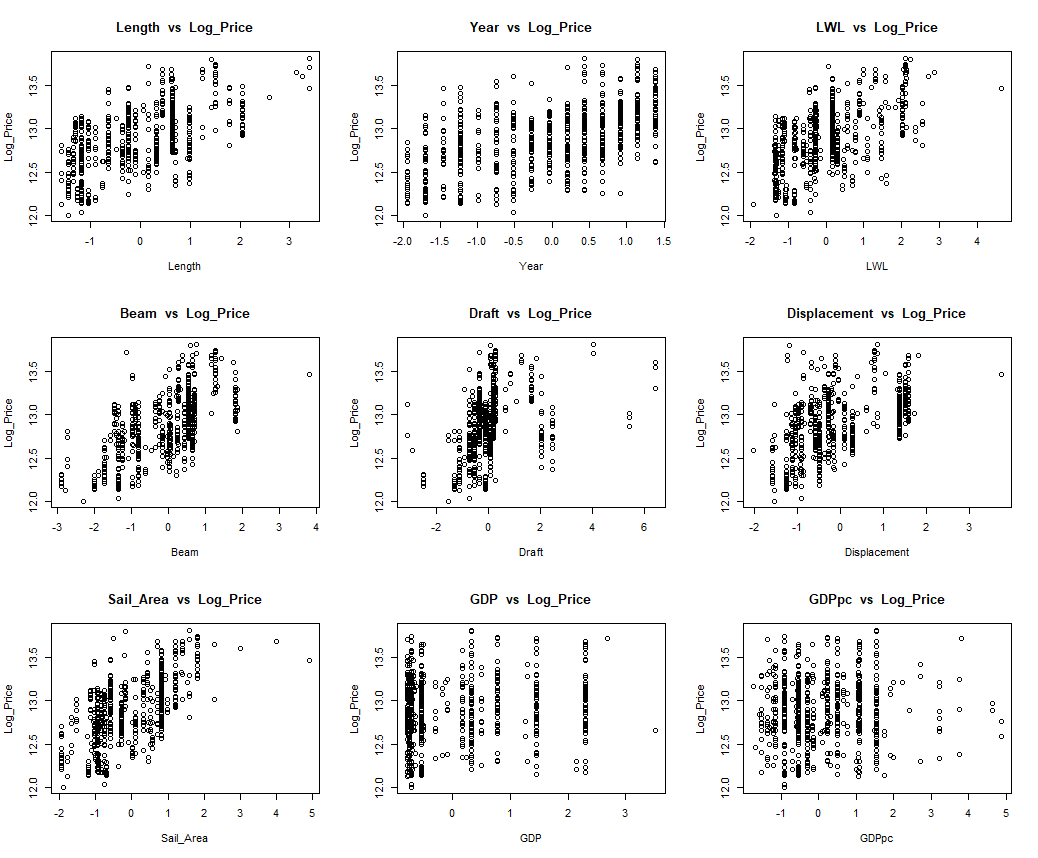
\includegraphics[width=0.6\textwidth]{res/sandian.png}
	\caption{变量散点图}
	\label{fig:sandian}
\end{figure}
不难发现,其中 Year 和 Draft 这两个解释变量与 Price 不止有简单的线性关系,所以我们不妨加入 $Year^2$ 和 $Draft^2$ 这两个二次解释变量,与其他九个一次项解释变量一同作为解释变量(共 11 个解释变量),进行线性回归模型 lr\_model01 的建立,并对模型效果进行查看,结果如下:\par 
\begin{table}[h]
	\centering
	\caption{lr\_model01 相关参数分析}\vspace{0.25\baselineskip}
	\begin{tabular}{@{}llllll@{}}
		\hline
		变量 & 估计系数 & 标准误 & t值 & p值 & 显著性 \\
		\hline
		常数 & 12.08259 & 0.04164 & 290.178 & < 2E-16 & *** \\
		Length & 0.53893 & 0.10232 & 5.267 & 1.720E-07 & *** \\
		Year & 0.33185 & 0.07746 & 4.284 & 2.020E-05 & *** \\
		Year2 & 0.33876 & 0.06940 & 4.881 & 1.240E-06 & *** \\
		LWL & 0.25419 & 0.11197 & 2.270 & 2.343E-02 & * \\
		Beam & 0.49083 & 0.08193 & 5.991 & 2.980E-09 & *** \\
		Draft & -0.51765 & 0.20442 & -2.532 & 1.150E-02 & * \\
		Draft2 & 0.66579 & 0.20017 & 3.326 & 9.150E-04 & *** \\
		Displacement & -0.07515 & 0.06755 & -1.112 & 2.663E-01 & \\
		Sail Area & 0.34450 & 0.10534 & 3.270 & 1.114E-03 & ** \\
		GDP & 0.14240 & 0.02557 & 5.569 & 3.350E-08 & *** \\
		GDP per capita & 0.10934 & 0.03991 & 2.740 & 6.263E-03 & ** \\
		\midrule
		R$^2$ = 0.7962& 调整R$^2$ = 0.7938& F(11,929) = 329.9& p < 2.2e-16& &\\ \bottomrule
		\end{tabular}
\end{table}
分析上述表格,由 $R^2$ 和调整 $R^2$ 值接近于 1,可知本模型拟合效果良好,且p 值小于 0.05,说明在检验水平为 0.05 条件下,因变量与其他变量之间的线性关系显著。
\subsection{模型改进}
由 lr\_model01 的相关参数分析表不难看出,Displacement 这一解释变量的显著性很低,为了增加模型的泛用性和鲁棒性,我们对此特征做删除处理。\par 
运用方差膨胀因子法对本模型进行多重共线性诊断,检验结果如下:\par 
\begin{table}[h]
	\centering
	\caption{方差膨胀因子法}\vspace{0.25\baselineskip}
	\begin{tabular}{ccccccc}
		\toprule
		变量 & Length & Year & Year2 & LWL & Beam & Draft \\
		vif值 & 15.217 & 20.963 & 20.162 & 10.647 & 5.510 & 16.486 \\
		\hline
		变量 & Draft2 & Displacement & Sail Area & GDP & GDP pc &\\
		vif值 & 14.614 & 5.230 & 8.150 & 1.396 & 1.409 &\\
		\bottomrule
	\end{tabular}
\end{table}
由检验结果知,解释变量 Length, LWL, Year, Year2, Draft, Draft2 之间存在严重的多重共线性,故将它们按照lr\_model01回归得到的权重进行合并,得到新的解释变量 LenLWL, Year12, Draft12。\par
最终使用LenLWL, Year12, Beam,Draft12, Sail\_Area, GDP,GDPpc 作为解释变量,继续以 Log\_Price 作为响应变量重新建模得到 lr\_model02。下面将展示对模型 lr\_model02 潜在问题的诊断及修正过程。
\subsection{模型诊断}
\subsubsection{整体诊断}
	\begin{figure}[H]
	\centering
	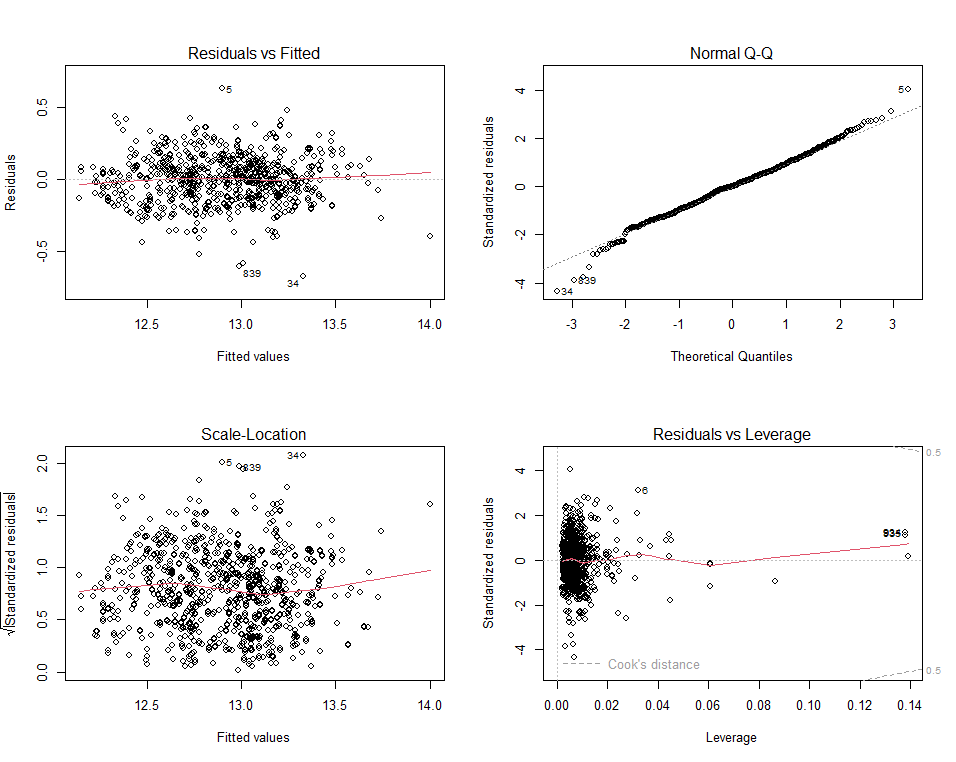
\includegraphics[width=0.8\textwidth]{res/zhenduan2.png}
	\caption{lr\_model02 模型诊断图}
	\label{fig:zhenduan2}
\end{figure}
绘制线性模型的整体散点图进行模型整体分析。观察左下图可知散点分布基本随机;观察Q-Q图可知,随横坐标增大,散点分散近似成一条直线,因此可认为残差服从正态分布;观察右下图可知存在较多离群点。下面将对模型进行检验。
\subsubsection{残差正态性检验}
由上面残差Q-Q图可直观判断,残差服从正态分布,下面针对模型lr\_model02的标准化残差进行K-S检验,检验结果如下。\par
\begin{table}[h]
	\centering
	\caption{K-S检验}
		\vspace{0.25\baselineskip}
	\begin{tabular}{ccc}
		\toprule
		检验变量 & 统计量D值 & P值 \\
		\hline
		lr\_model02 模型残差(标准化) & 0.040816 & 0.08696 \\
		\bottomrule
	\end{tabular}
\end{table}
由检验结果,检验 p 值并不显著,因此在检验水平为 0.05 条件下不能拒绝原假设,即模型 lr\_model02 的标准化残差服从正态分布。
\subsubsection{方差齐性检验}
由整体检验时已经分析残差图,散点随机性较良好,因此直观认为残差之间不存在异方差,对模型采用 ncv 计分检验,检验结果如下表。\par 
\begin{table}[h]
	\centering
	\caption{ncv计分检验}
		\vspace{0.25\baselineskip}
\begin{tabular}{cccc}
	\toprule
	检验变量 & Chisquare & df & p \\
	\hline
	lr\_model02 & 0.872637 & 1 & 0.35023 \\
	\bottomrule
\end{tabular}
\end{table}

由检验 p 值大于0.05可认为检验不显著,则认为不存在异方差。
\subsubsection{多重共线性诊断}
运用方差膨因子法对模型 lr\_model02 进行多重共线性诊断,结果如下:\par 
\begin{table}[htbp]
	\centering
	\caption{方差膨胀因子法}\vspace{0.25\baselineskip}
	\begin{tabular}{cccccc}
		\toprule
		变量 & Len LWL & Year12 & Beam & Draft12 & \\
		vif值 & 8.238574 & 1.139205 & 4.874397 & 1.243277 & \\
		\midrule
		变量 & Sail Area & GDP & GDP pc & & \\
		vif值 & 4.655615 & 1.38501 & 1.404301 & & \\
		\bottomrule
	\end{tabular}%
	\label{tab:my_label}%
\end{table}
由检验结果知,各解释变量之间不存在严重的多重共线性,即多重共线性检验通过。

\subsubsection{模型应用}
经上述检验,可确定最终模型 lr\_model02 ,对其效果进行查看,结果如下。\par 
\begin{table}[h]
	\centering
	\caption{lr\_model02 相关参数分析}\vspace{0.25\baselineskip}
	\label{tab:lr_model02}
	\begin{tabular}{llllll}
		\hline
		变量 & 估计系数 & 标准误 & t值 & p值 & 显著性 \\ \hline
		常数 & 12.908192 & 0.005075 & 2543.432 & $<$ 2e-16 & *** \\
		Len LWL & 0.143063 & 0.014564 & 9.823 & $<$ 2e-16 & *** \\
		Year12 & 0.209391 & 0.005416 & 38.665 & $<$ 2e-16 & *** \\
		Beam & 0.069463 & 0.01151 & 6.035 & 2.29E-09 & *** \\
		Draft12 & 0.023667 & 0.005658 & 4.183 & 3.15E-05 & *** \\
		Sail Area & 0.039203 & 0.011575 & 3.387 & 0.000737 & *** \\
		GDP & 0.033562 & 0.005943 & 5.648 & 2.16E-08 & *** \\
		GDP per capita & 0.016561 & 0.006028 & 2.747 & 0.006126 & ** \\ \hline
		R$^2$ = 0.7958 & 调整R$^2$ = 0.7942 & F(7,933) = 519.3 & p $<$ 2.2e-16 & & \\ \hline
	\end{tabular}
\end{table}
由于合并解释变量前我们已经对解释变量进行了标准化处理,且按照原模型中其对应的权重进行合并,合并后再次进行标准化处理,且被删除的Displacement 这一解释变量的显著性很低,所以$R^2$与调整$R^2$的值未出现较大变化,lr\_model02 的 $R^2$ 和调整 $R^2$ 均大于线性回归模型 lm2 和对数线性回归模型 model1,且 p 值仍旧显著,证明模型基本可靠。建模最终得到回归方程:\par 
\begin{align}
	ln_y^{*}= &12.908192+(1.552e-02) x_1+(4.585e-02) x_2+(6.435e-03) \nonumber \\
	&\quad x_2^2+(5.551e-03) x_3+(6.946e-02) x_4+(-2.045e-04) x_5+(1.727e-04) \nonumber \\
	&\quad x_5^2+(3.920e-02) x_7+(3.356e-02) x_8+(1.656e-02) x_9
\end{align}
模型输出的因变量为价格的对数,在进行预测错误率计算之前,需要将其通过指数函数转化为价格数据,以此代入上述回归方程进行计算。计算出该对数线性回归模型的预测错误率为r=12.08\%,相较于线性回归模型和对数线性回归模型略有改善,可见此广义线性回归模型对数据预测的准确性略有提升,但受限于线性模型的局限性,很难实现大幅改进。
\section{总结与反思}
针对此数据集,我们分别建立了简单线性回归、对数线性回归与广义对数线性回归模型,并对模型进行多角度效果评价,最终发现广义线性回归模型对数据的解释与预测效果最优,说明变量之间的相关性并不能仅被线性表示。

\end{document}